\documentclass[aspectratio=169]{beamer}
\beamertemplatenavigationsymbolsempty
\usecolortheme{beaver}
\setbeamertemplate{blocks}[rounded=true, shadow=true]
\setbeamertemplate{footline}[page number]


\usepackage{graphicx}
\usepackage{amsmath}
\usepackage{amsfonts}
\usepackage{caption}
\usepackage{subcaption}
\usepackage{float}
\usepackage[english,russian]{babel}


\usepackage[utf8]{inputenc}
\usepackage{amssymb,amsfonts,amsmath,mathtext}
%\usepackage{subfig}
\usepackage{tikz}
\usepackage{xcolor}
\usepackage[all]{xy} % xy package for diagrams
\usepackage{array}
\usepackage{multicol}% many columns in slide
\usepackage{hyperref}% urls
\usepackage{hhline}%tables


\def\bw{\mathbf{w}}
\def\balpha{\boldsymbol{\alpha}}

% Your figures are here:
\graphicspath{ {fig/} {../fig/} }

\definecolor{ao(english)}{rgb}{0.0, 0.5, 0.0}
\definecolor{bleudefrance}{rgb}{0.19, 0.55, 0.91}

%----------------------------------------------------------------------------------------------------------
\title[\hbox to 56mm{Feature generation}]{Поиск согласованных нейросетевых моделей в задаче мультидоменного обучения}
\author{К.\,Д.~Яковлев\inst{1} \and \and О.\,Ю.~Бахтеев\inst{1,2}\and В.\,В.~Стрижов\inst{1,2} \\
\tt{\footnotesize \{iakovlev.kd, bakhteev, strijov\}@phystech.edu }}
\institute{\inst{1} Москва, Московский физико-технический институт \and
\inst{2} Москва, Вычислительный центр им. А.А. Дородницына ФИЦ ИУ РАН} \date{2022}
%----------------------------------------------------------------------------------------------------------
\begin{document}
%----------------------------------------------------------------------------------------------------------
\begin{frame}
\thispagestyle{empty}
\maketitle
\end{frame}
%-----------------------------------------------------------------------------------------------------
\begin{frame}{Цель исследования}

\begin{block}{Цель} 
  Предложить метод поиска архитектуры модели глубокого обучения в задаче мультидоменного
  обучения.
\end{block}

~\\
\begin{block}{Проблема}
  Модели, не учитывающие разделение выборки на домены, имеют низкую обобщающую способность.
\end{block}
~\\
\begin{block}{Метод решения}
  Предлагаемый метод основан на построении мультимодели. Для каждого домена оптимизируется
  отдельная структура. Также предлагаются два метода регуляризации: структурная и
  регуляризация пространства скрытых представлений модели.
\end{block}

\end{frame}

%----------------------------------------------------------------------------------------------------------


\begin{frame}{Основная литература}
\begin{thebibliography}{1}


\bibitem{darts} 
Hanxiao Liu and Karen Simonyan and Yiming Yang. 
\textit{DARTS: Differentiable Architecture Search}.
CoRR, 2018.


\bibitem{wang2021multi}
Wang, Q., Ke, J., Greaves, J., Chu, G.,
Bender, G., Sbaiz, L., Go, A., Howard, A., Yang, M.,
Gilbert, J. \& Others
\textit{Multi-path neural networks for on-device multi-domain visual classification}.
CoRR, 2021.

\bibitem{darts-cc}
Yakovlev, K., Grebenkova, O., Bakhteev, O. \& Strijov, V.
\textit{Neural Architecture Search with Structure Complexity Control}.
CoRR, 2022.



\end{thebibliography}	
\end{frame}

\begin{frame}{Постановка задачи поиска архитектуры}
\begin{itemize}
\item Архитектура модели представляет собой ориентированный ациклический граф. Каждому ребру ставится в соответствие отображение $\boldsymbol{g}^{(i, j)}$, причем
\[
\boldsymbol x^{(j)} = \sum_{i < j}\boldsymbol{g}^{(i, j)}(\boldsymbol{x}^{(i)}).
\]
\item Пусть вектор $\vec{\boldsymbol g}^{(i, j)}$ -- вектор, составленный из доступных для ребра $(i, j)$ отображений. Пусть вектор $\boldsymbol\alpha^{(i, j)}$ -- вектор структурных параметров. Смешанная операция
\[
\hat{\boldsymbol g}^{(i, j)}(\boldsymbol x^{(i)}) = \langle\boldsymbol{softmax}(\boldsymbol \alpha^{(i, j)}), \vec{\boldsymbol g}^{(i, j)}(\boldsymbol{x}^{(i)})\rangle.
\]
\item Задана выборка $\mathfrak{D} = \mathfrak{D}_\text{train} \cup \mathfrak{D}_\text{val}$. Задана функция потерь $\mathcal{L}_\text{train}, ~\mathcal{L}_\text{val}$. Пусть $\boldsymbol\alpha = [\boldsymbol\alpha^{(i, j)}]$. Пусть $\boldsymbol w$ -- параметры модели. Двухуровневая задача оптимизации
\[
\min_{\boldsymbol\alpha}\mathcal{L}_\text{val}(\boldsymbol w^*, \boldsymbol\alpha),
\]
\[
\mathrm{s.t.} ~~\boldsymbol w^* = \arg\min_{\boldsymbol w}\mathcal{L}_\text{train}(\boldsymbol w, \boldsymbol\alpha)
\]
\end{itemize}
\end{frame}


\begin{frame}{Архитектура модели}
\begin{figure}
\centering
\begin{minipage}{.5\textwidth}
  \centering
  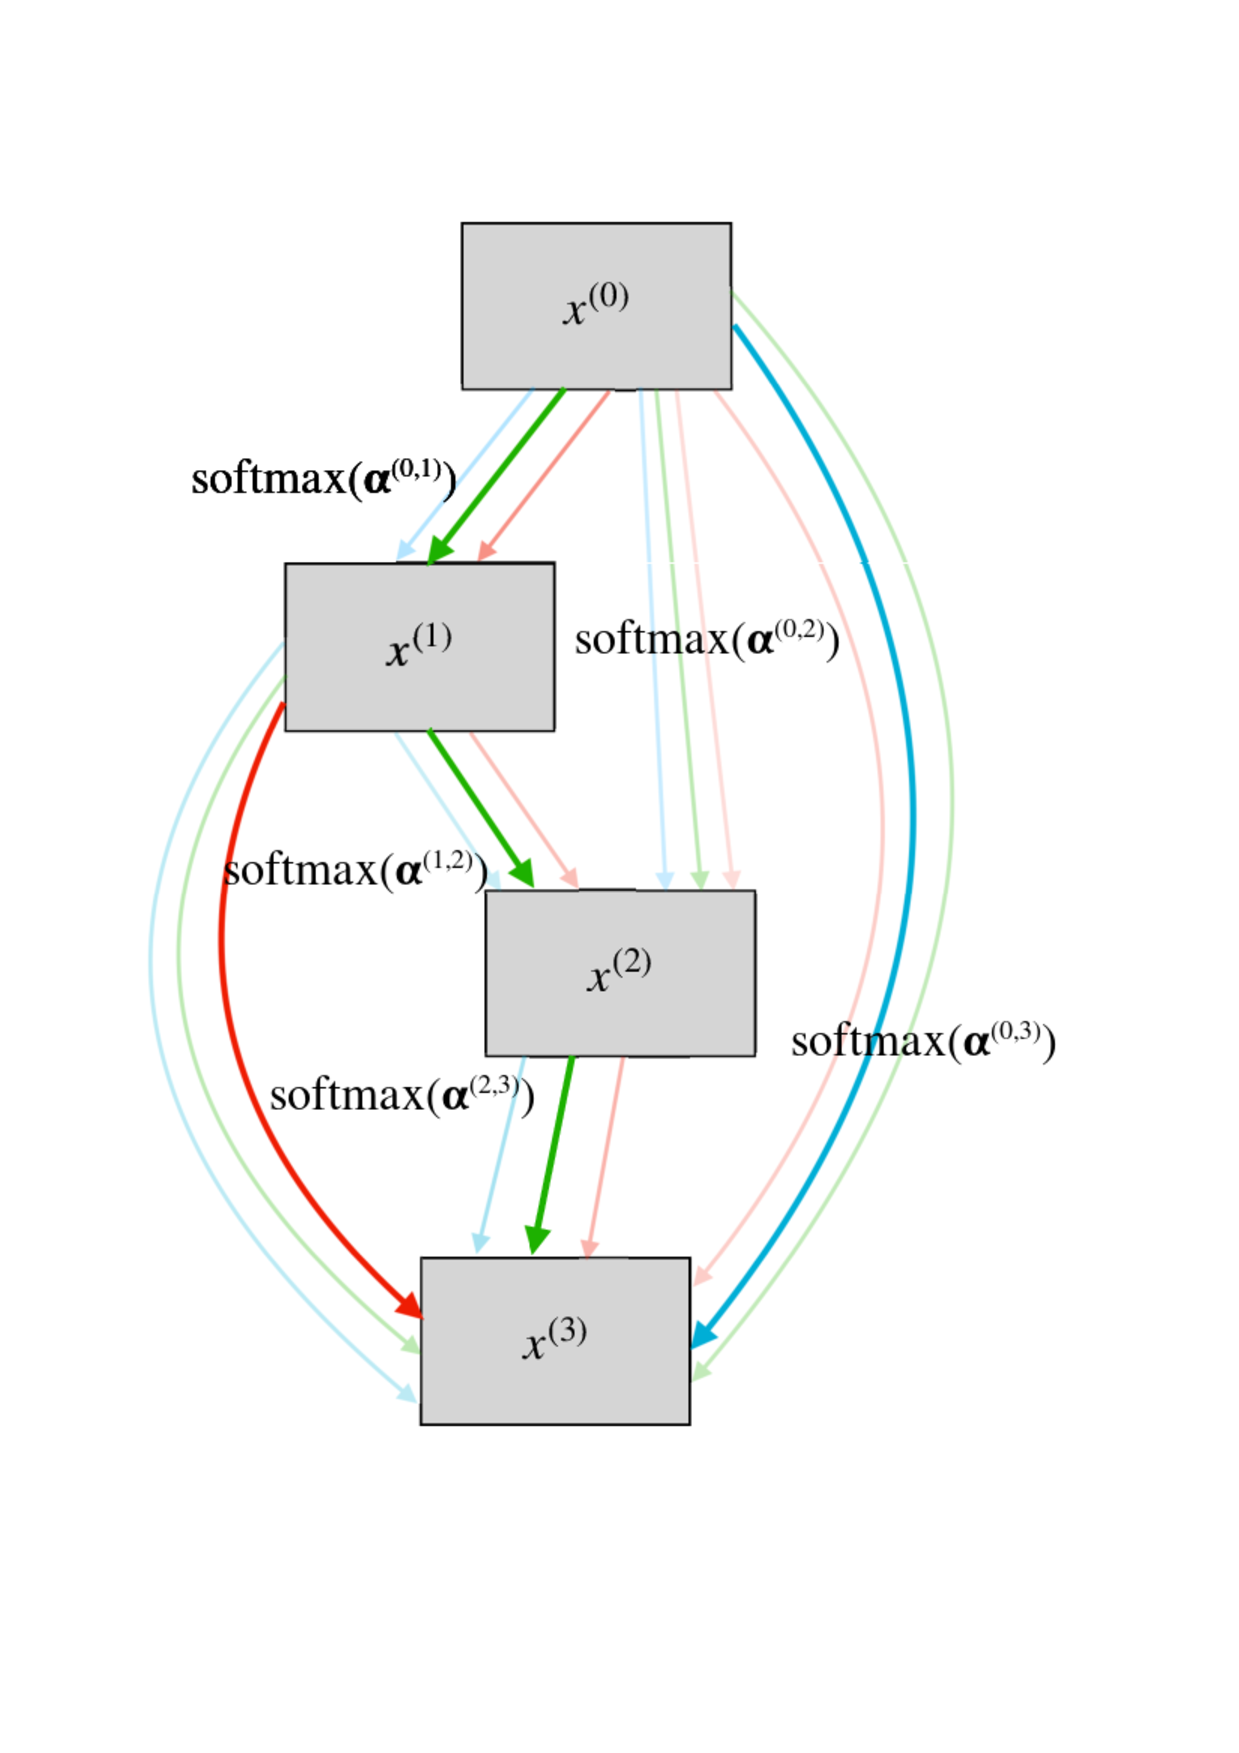
\includegraphics[width=.7\linewidth]{Graph_no_lambda.pdf}
\end{minipage}%
\begin{minipage}{.5\textwidth}
\begin{itemize}
\item Смешанная операция:
\[
\hat{\boldsymbol g}^{(i, j)} = {\color{red}{\text{softmax}(\boldsymbol\alpha^{(i, j)})_1\boldsymbol{g}^{(i, j)}_1(\boldsymbol x^{(i)})}} + 
\]
\[
{\color{ao(english)}{\text{softmax}(\boldsymbol\alpha^{(i, j)})_2\boldsymbol{g}^{(i, j)}_2(\boldsymbol x^{(i)})}} + 
\]
\[
{\color{bleudefrance}{\text{softmax}(\boldsymbol\alpha^{(i, j)})_3\boldsymbol{g}^{(i, j)}_3(\boldsymbol x^{(i)})}} 
\]
\end{itemize}
 
\end{minipage}%
\end{figure}
\end{frame}


\begin{frame}{Постановка задачи поиска архитектуры на мультидоменных данных}
  \begin{itemize}
    \item 
    Задано $D$ доменов, $\{\mathfrak{D}_d\}_{d=1}^D, ~\mathfrak{D}_d = (\mathbf{X}_d, \mathbf{y}_d),
    ~\mathbf{y}_d \subset \mathcal{Y}$.
    Пусть заданы функции потерь $\mathcal{L}_\text{train}^{(d)}$ и $\mathcal{L}_\text{val}^{(d)}$.
    Модель задается разделяемыми между доменами параметрами $\bw$. Пусть $\balpha_d$ -- вектор
    структурных параметров домена $d$, $\balpha = [\balpha_d]_{d=1}^D$.
    \item Задано распределение на доменах $d \sim \mathrm{Categorical}(\mathbf{p})$.
    Двухуровневая задача оптимизации

    \begin{align*}
      \boldsymbol\alpha^* = \arg\min_{\boldsymbol\alpha}
      \sum_{d=1}^Dp_d\mathcal{L}_\text{valid}^{(d)}(\mathbf{w}^*,\boldsymbol\alpha_d),\\
      \mathrm{s.t.} \quad \mathbf{w}^* = \arg\min_{\mathbf{w}}\sum_{d=1}^D
      p_d\mathcal{L}_\text{train}^{(d)}(\mathbf{w}, \boldsymbol\alpha_d).
    \end{align*}

    \item Получение итоговой архитектуры для каждого из доменов:
    \begin{align*}
      \mathbf{g}^{(i, j)}(.) = \vec{\mathbf{g}}^{(i, j)}_{k^*}, \quad k^* = \arg\max_k (\alpha^{(i, j)}_d)_k.
    \end{align*}
    

    \end{itemize}
\end{frame}




\begin{frame}{Предлагаемые регуляризаторы}
\begin{itemize}
\item Заданы распределения на ребрах графа
$P_d^{(i, j)} = \mathrm{Categorical}(\mathbf{softmax}(\balpha^{(i, j)}_d))$. Структурный
регуляризатор:
\begin{align*}
  \mathcal{L}_\text{struct}(\boldsymbol\alpha) = \frac{1}{D(D-1)}\sum_{(i, j)}
  \sum_{d=1}^D\sum_{d'=1, ~d' \not= d}^D\mathrm{JS}(P_d^{(i, j)}||P_{d'}^{(i, j)}),
\end{align*}
где $\mathrm{JS}(.||.)$ -- дивергенция Йенсена—Шеннона.
\item Заданы наборы объектов для каждого из доменов $\{\mathcal{S}_b^{(d)}\}_{d=1}^D$
Регуляризатор пространства скрытых представлений модели:
\begin{align*}
  \mathcal{L}_\text{contr}(\mathbf{w}, \boldsymbol\alpha) = \mathsf{E}_{d, d' \sim \mathrm{Categorical}(\mathbf{p})}
  \mathsf{E}_{\mathcal{S}_b^{(d)}, \mathcal{S}_b^{(d')}}\mathcal{L}_\text{triplet}
  (\mathbf{w}, \boldsymbol\alpha, \mathcal{S}_b^{(d)}, \mathcal{S}_b^{(d')}),
\end{align*}
где $\mathcal{L}_\text{triplet}$ -- триплетная функция потерь для скрытых представлений 
$\mathcal{S}_b^{(d)}, \mathcal{S}_b^{(d')}$.

\end{itemize}
\end{frame}



\begin{frame}{Построение мультимодели}

\begin{figure}
\centering
\begin{minipage}{.4\textwidth}
  \centering
  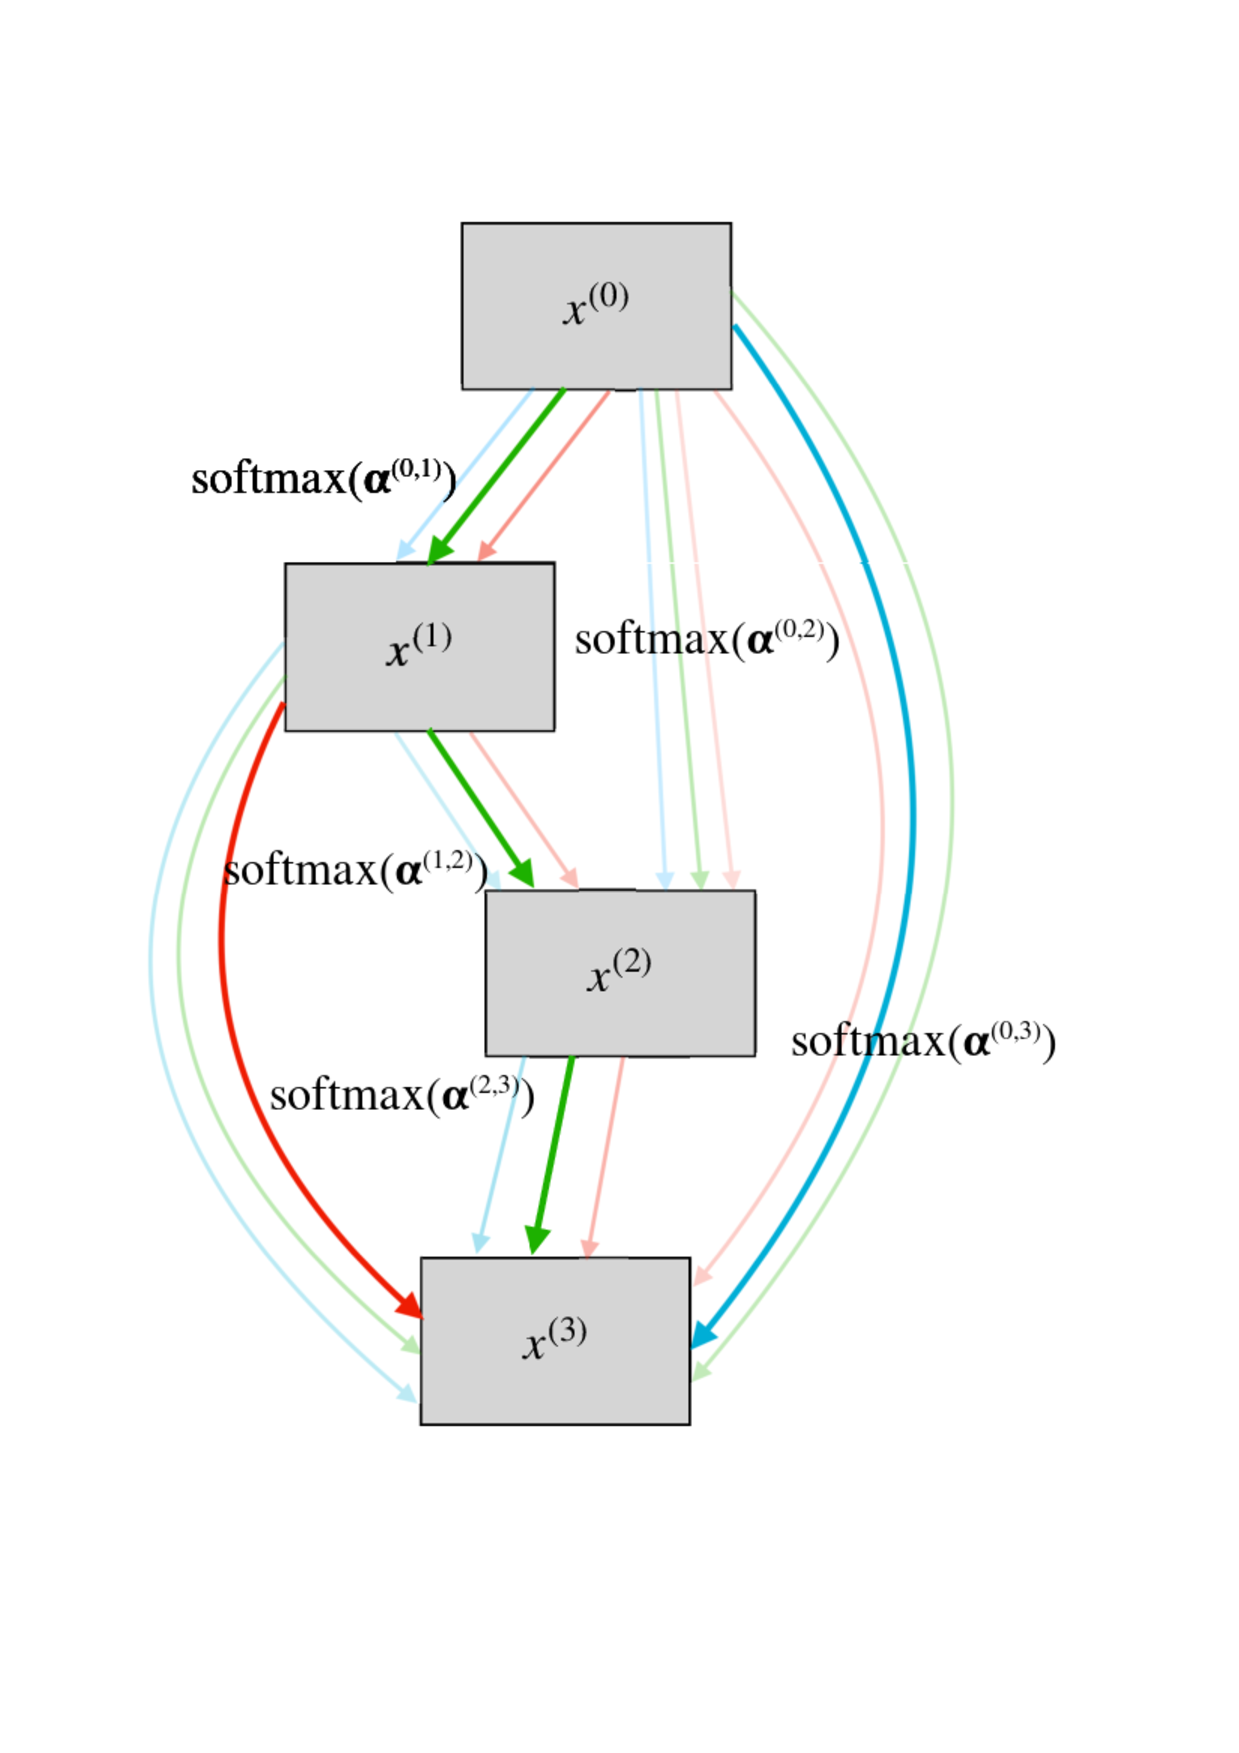
\includegraphics[width=.9\linewidth]{Graph_no_lambda.pdf}
\end{minipage}%
\begin{minipage}{.6\textwidth}
  \centering
  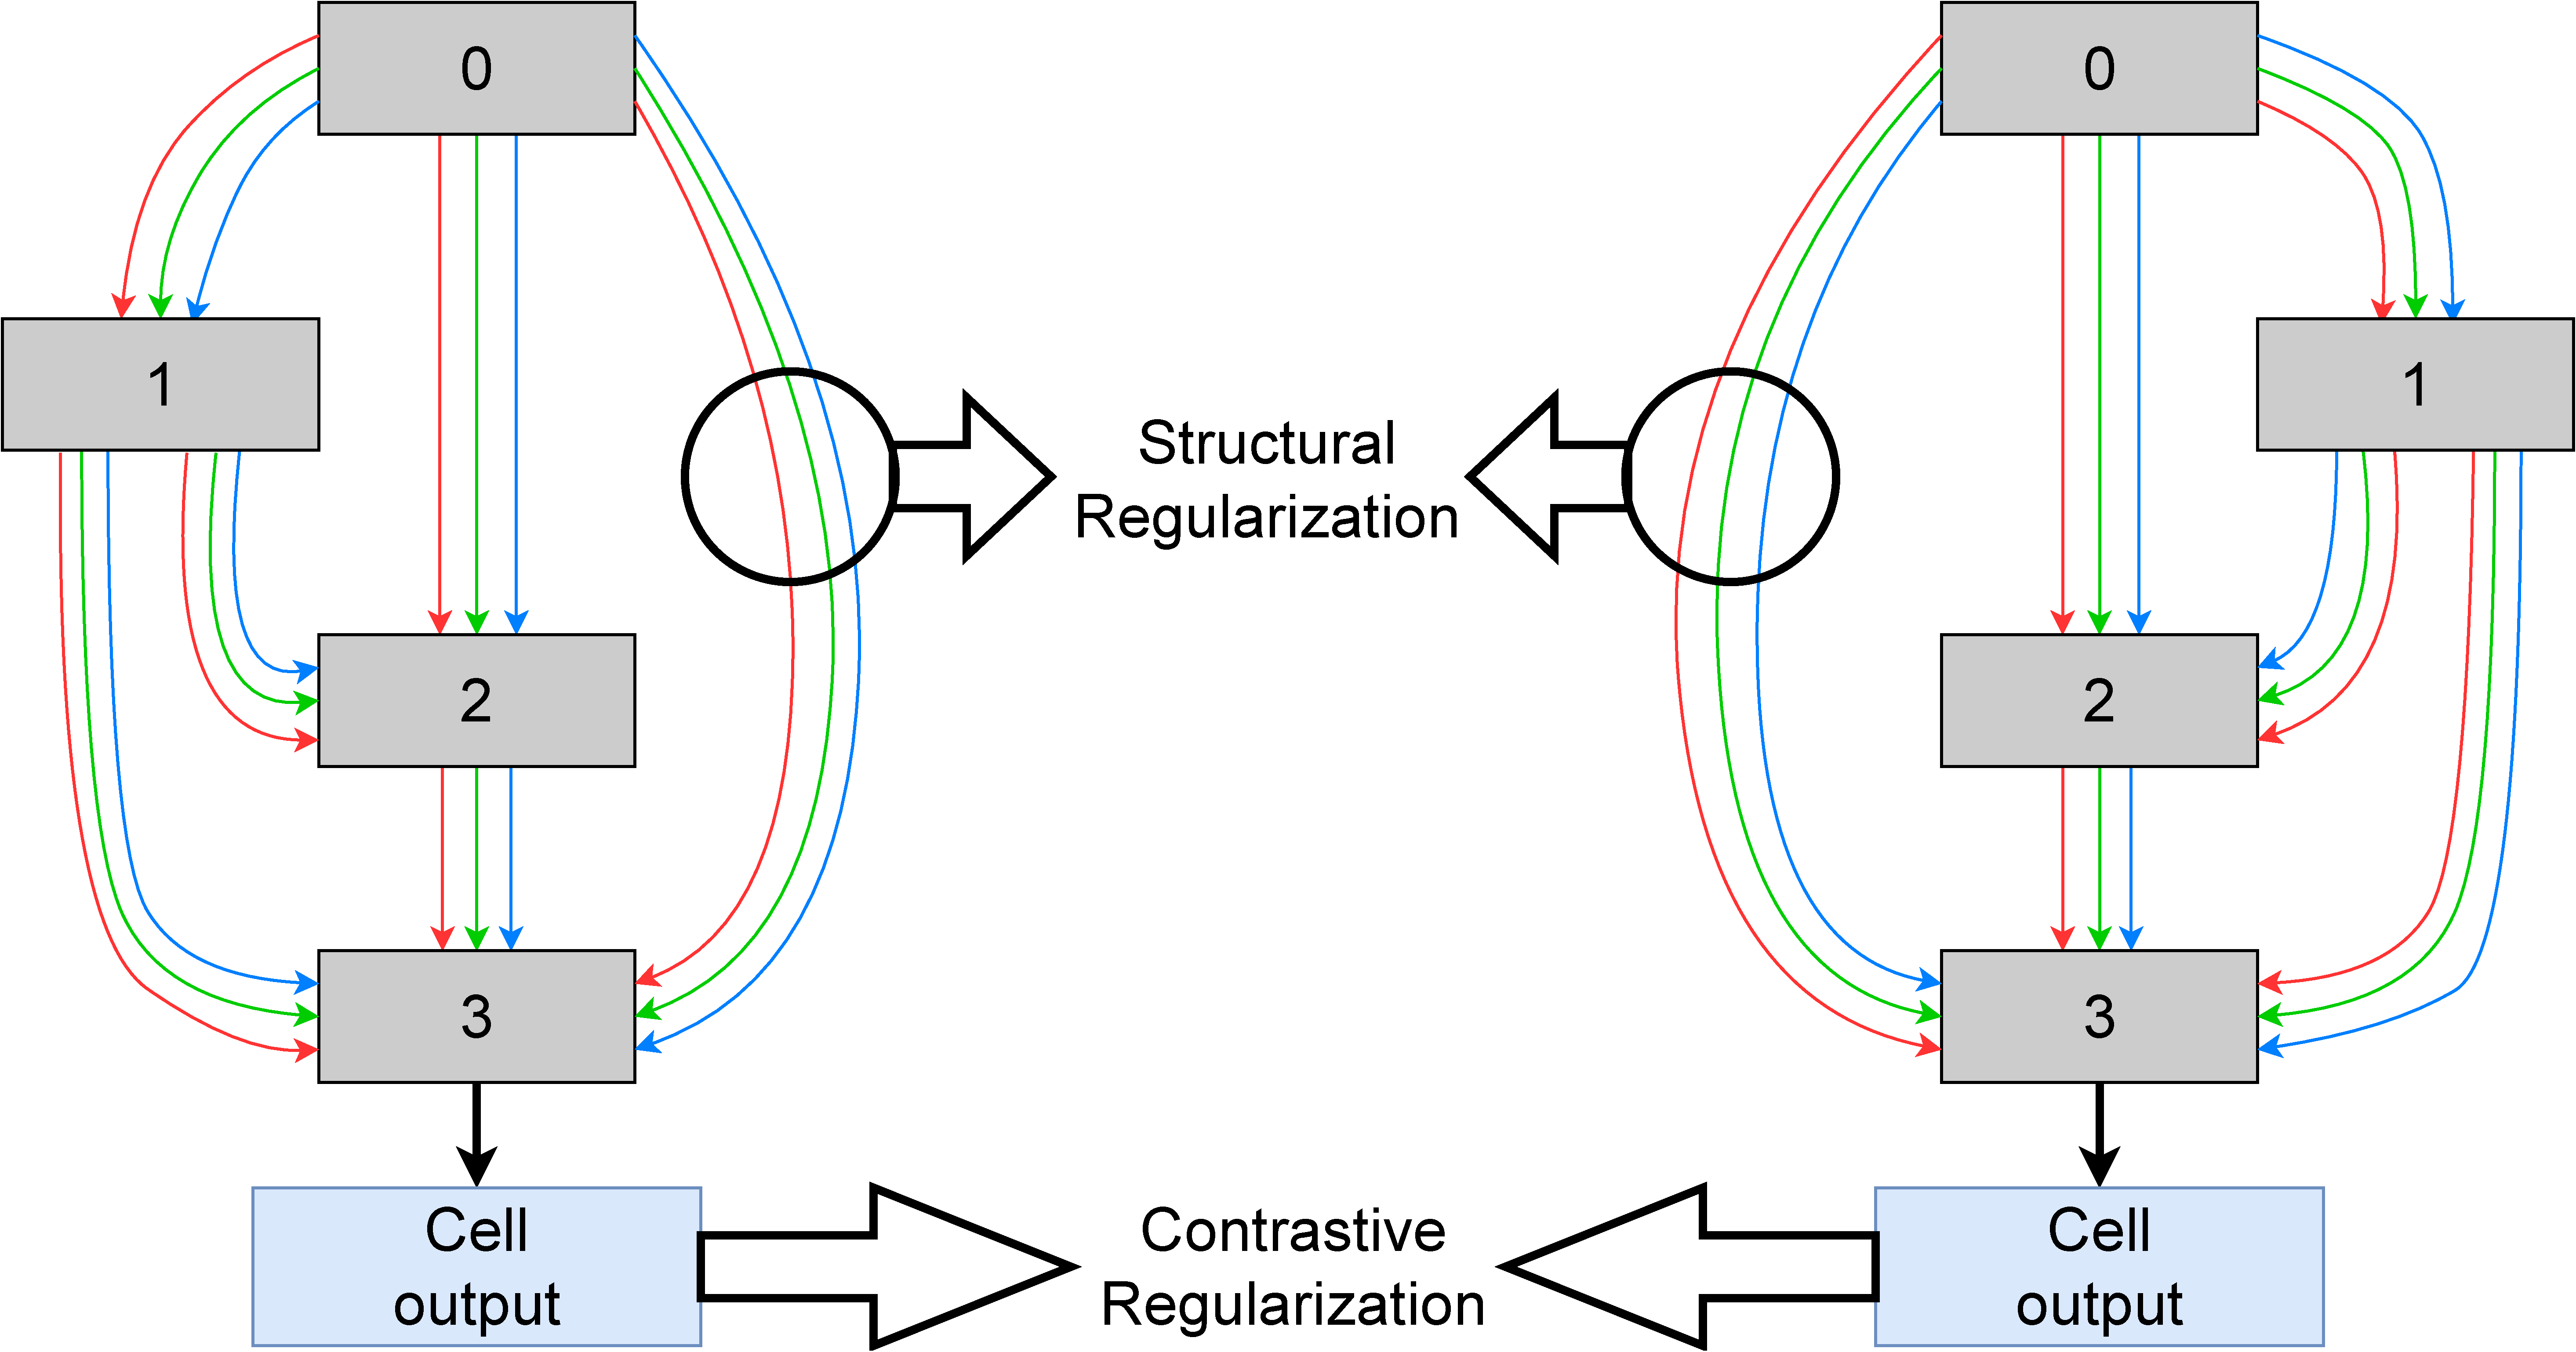
\includegraphics[width=1.0\linewidth]{multimodel_reg.pdf}
\end{minipage}%
\end{figure}
\end{frame}




\begin{frame}{Задача оптимизации}
\begin{itemize}
  \item Заданы коэффициенты регуляризации $\beta_\text{trip} \geq 0, ~\beta_\text{struct} \geq 0$.
  Оптимальный вектор структурных параметров в задаче выбора архитектуры на мультидоменных
  данных находится из следующей задачи оптимизации:
  \begin{align*}
    \boldsymbol\alpha^* &= \arg\min_{\boldsymbol\alpha}\sum_{d=1}^Dp_d
    \mathcal{L}_\text{val}^{(d)}(\bw^*, \boldsymbol\alpha) + 
    \beta_\text{trip}\mathcal{L}_\text{contr}(\bw, \balpha) + 
    \beta_\text{struct}\mathcal{L}_\text{struct}(\balpha)
    ,\\
    \mathrm{s.t.}\quad \bw^* &= \arg\min_{\bw}\sum_{d=1}^Dp_d
    \mathcal{L}_\text{train}^{(d)}(\bw, \balpha) +
    \beta_\text{trip}\mathcal{L}_\text{contr}(\bw, \balpha).
  \end{align*}
  
\end{itemize}
\end{frame}




\begin{frame}{Постановка вычислительного эксперимента}

\begin{itemize}
\item Цель -- получение зависимости качества работы мультимодели и
количества ее параметров в зависимости от используемого регуляризатора.
\item Эксперимент проводится на подвыборке MNIST. В качестве доменов рассматриваются
изображения, повернутые на угол, кратный $\pi/2$. Число доменов меняется от 1 до 4.
 Сравниваются следующие модели:
мультимодель со структурной регуляризацией, мультимодель с регуляризацией скрытых представлений,
а также модель, не учитывающая разбиение выборки на домены.
\item Оценивается средняя точность (accuracy) на тестовой выборке для каждого из доменов.
Также приводится количество параметров для каждой модели.
\end{itemize}

\end{frame}


\begin{frame}{Результаты вычислительного эксперимента}
  \begin{table}[h!]
    \centering
     \begin{tabular}{||c c c||}
     \hline
     model & accuracy & num. of params \\ [0.5ex] \hline\hline
     \multicolumn{3}{|| c ||}{1 domain} \\
      single & 60.59 & 5029 \\ \hline \hline 

     \multicolumn{3}{|| c ||}{2 domains} \\
     single, union & 66.95 & 6560 \\
     multimodel, struct & 62.86 & \textbf{5248} \\
     multimodel, contr & \textbf{69.64} & 9328 \\
     \hline \hline

     \multicolumn{3}{|| c ||}{3 domains} \\
     single, union & 63.02 & 5685\\
     multimodel, struct & 64.85 & \textbf{6826}\\
     multimodel, contr & \textbf{65.01} & 12096 \\
     \hline\hline

     \multicolumn{3}{|| c ||}{4 domains} \\
     single, union & 67.16 & 6560\\
     multimodel, struct & 63.15 & \textbf{7872}\\
     multimodel, contr & \textbf{67.98} & 13685 \\
     \hline\hline
     \end{tabular}
    \end{table}
\end{frame}



\begin{frame}{Заключение}
    \begin{itemize}
    \item Рассмотрена задача поиска архитектуры модели глубокого
    обучения на мультидоменных данных. Задача рассматривалась как
    задача мультимоделирования.
    \item Предложены два метода регуляризации: регуляризация структуры и регуляризация
    пространства скрытых представлений модели.
    \item Продемонстрирована работоспособность предлагаемого решения. При использовании
    первого регуляризатора мультимодель имеет меньшее число параметров. При использовании
    второго регуляризатора модель имеет лучшую точность классификации.
    \item В дальнейшем планируется провести вычислительный эксперимент на задаче
    мультиязычного языкового моделирования.
    \end{itemize}
\end{frame}

%----------------------------------------------------------------------------------------------------------
\end{document} 